\documentclass[tikz,border=2pt]{standalone}
\usepackage{tikz}
\usetikzlibrary{shapes,arrows.meta,positioning,calc,fit,backgrounds}
\usepackage{amsmath,amssymb}

\begin{document}
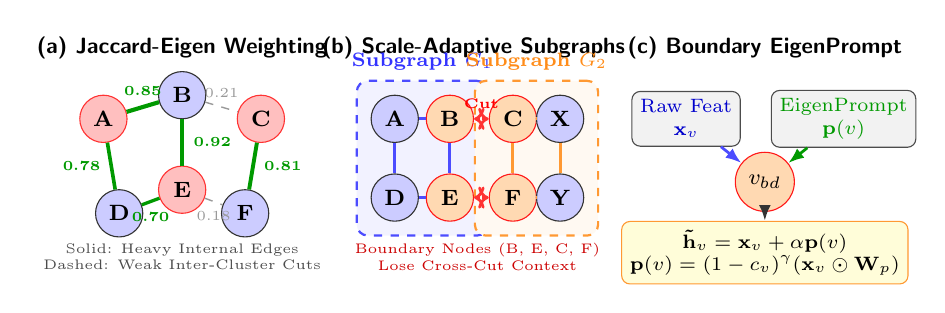
\begin{tikzpicture}[
    font=\sffamily\footnotesize,
    node distance=1.2cm,
    node/.style={circle, draw=black!80, fill=blue!20, minimum size=6mm, inner sep=0pt, font=\bfseries\footnotesize},
    highc/.style={circle, draw=red!80, fill=red!25, minimum size=6mm, inner sep=0pt, font=\bfseries\footnotesize},
    bound/.style={circle, draw=red!90, fill=orange!30, minimum size=6mm, inner sep=0pt, font=\bfseries\footnotesize},
    part1/.style={rounded corners=4pt, draw=blue!70, fill=blue!5, dashed, line width=0.8pt},
    part2/.style={rounded corners=4pt, draw=orange!80, fill=orange!5, dashed, line width=0.8pt},
    box/.style={draw=black!70, fill=gray!10, rounded corners=3pt, inner sep=3pt, align=center, font=\scriptsize}
]

% ---------------- (a) Spectral Edge Weighting ----------------
\begin{scope}[local bounding box=subfigA]
    \node at (1.2, 2.7) {\textbf{(a) Jaccard-Eigen Weighting}};
    \node[highc] (a1) at (0.2, 1.8) {A};
    \node[node]  (b1) at (1.2, 2.1) {B};
    \node[highc] (c1) at (2.2, 1.8) {C};
    \node[node]  (d1) at (0.4, 0.6) {D};
    \node[highc] (e1) at (1.2, 0.9) {E};
    \node[node]  (f1) at (2.0, 0.6) {F};

    \draw[line width=1.5pt, green!60!black] (a1) -- node[above, font=\tiny\bfseries] {0.85} (b1);
    \draw[line width=0.5pt, black!40, dashed] (b1) -- node[above, font=\tiny] {0.21} (c1);
    \draw[line width=1.3pt, green!60!black] (a1) -- node[left, font=\tiny\bfseries] {0.78} (d1);
    \draw[line width=1.6pt, green!60!black] (b1) -- node[right, font=\tiny\bfseries] {0.92} (e1);
    \draw[line width=1.4pt, green!60!black] (c1) -- node[right, font=\tiny\bfseries] {0.81} (f1);
    \draw[line width=1.2pt, green!60!black] (d1) -- node[below, font=\tiny\bfseries] {0.70} (e1);
    \draw[line width=0.5pt, black!40, dashed] (e1) -- node[below, font=\tiny] {0.18} (f1);

    \node[font=\tiny, align=center, text=black!70] at (1.2, 0.05) {Solid: Heavy Internal Edges\\Dashed: Weak Inter-Cluster Cuts};
\end{scope}

% ---------------- (b) Scale-Adaptive Partitions ----------------
\begin{scope}[xshift=3.7cm, local bounding box=subfigB]
    \node at (1.2, 2.7) {\textbf{(b) Scale-Adaptive Subgraphs}};

    % Partition 1
    \node[node]  (a2) at (0.2, 1.8) {A};
    \node[bound] (b2) at (0.9, 1.8) {B};
    \node[node]  (d2) at (0.2, 0.8) {D};
    \node[bound] (e2) at (0.9, 0.8) {E};

    \draw[line width=1.0pt, blue!70] (a2) -- (b2);
    \draw[line width=1.0pt, blue!70] (a2) -- (d2);
    \draw[line width=1.0pt, blue!70] (b2) -- (e2);
    \draw[line width=1.0pt, blue!70] (d2) -- (e2);

    \begin{scope}[on background layer]
        \node[part1, fit=(a2)(b2)(d2)(e2), inner sep=5pt] (p1) {};
    \end{scope}
    \node[font=\scriptsize\bfseries, blue!80, anchor=south] at (p1.north) {Subgraph $G_1$};

    % Partition 2
    \node[bound] (c2) at (1.7, 1.8) {C};
    \node[node]  (x2) at (2.3, 1.8) {X};
    \node[bound] (f2) at (1.7, 0.8) {F};
    \node[node]  (y2) at (2.3, 0.8) {Y};

    \draw[line width=1.0pt, orange!80] (c2) -- (x2);
    \draw[line width=1.0pt, orange!80] (c2) -- (f2);
    \draw[line width=1.0pt, orange!80] (x2) -- (y2);
    \draw[line width=1.0pt, orange!80] (f2) -- (y2);

    \begin{scope}[on background layer]
        \node[part2, fit=(c2)(x2)(f2)(y2), inner sep=5pt] (p2) {};
    \end{scope}
    \node[font=\scriptsize\bfseries, orange!90, anchor=south] at (p2.north) {Subgraph $G_2$};

    % Cut edge arrow
    \draw[<->, line width=1.0pt, red!80, densely dotted] (b2) -- node[above, font=\tiny\bfseries, red] {Cut} (c2);
    \draw[<->, line width=1.0pt, red!80, densely dotted] (e2) -- (f2);

    \node[font=\tiny, align=center, text=red!80!black] at (1.25, 0.05) {Boundary Nodes (B, E, C, F)\\Lose Cross-Cut Context};
\end{scope}

% ---------------- (c) Boundary EigenPrompt Bridging ----------------
\begin{scope}[xshift=7.4cm, local bounding box=subfigC]
    \node at (1.2, 2.7) {\textbf{(c) Boundary EigenPrompt}};

    \node[box, text=blue!80!black] (raw) at (0.2, 1.8) {Raw Feat\\$\mathbf{x}_v$};
    \node[box, text=green!60!black] (prm) at (2.2, 1.8) {EigenPrompt\\$\mathbf{p}(v)$};

    \node[bound, minimum size=7.5mm] (vbd) at (1.2, 1.0) {$v_{bd}$};

    \draw[-{Latex[length=2mm]}, line width=1.0pt, blue!70] (raw) -- (vbd);
    \draw[-{Latex[length=2mm]}, line width=1.0pt, green!60!black] (prm) -- (vbd);

    \node[box, fill=yellow!15, draw=orange!80, font=\scriptsize\bfseries] (out) at (1.2, 0.1) {
        $\mathbf{\tilde{h}}_v = \mathbf{x}_v + \alpha \mathbf{p}(v)$\\
        $\mathbf{p}(v) = (1 - c_v)^\gamma (\mathbf{x}_v \odot \mathbf{W}_p)$
    };
    \draw[-{Latex[length=2mm]}, line width=1.0pt, black!80] (vbd) -- (out);
\end{scope}

\end{tikzpicture}
\end{document}
